% -------------------------------------------------
% Anexo D. Interfaces del módulo de Escucha Activa
% -------------------------------------------------
\section*{Anexo D. Interfaces del módulo de Escucha Activa}
\addcontentsline{toc}{section}{Anexo D. Interfaces del módulo de Escucha Activa}
\label{anexo:interfaces_escucha_activa}

Este anexo presenta las interfaces asociadas al módulo de escucha activa. Las figuras ilustran los distintos momentos de interacción del estudiante durante una sesión de juego: la configuración inicial, la selección y gestión de sesiones, el desarrollo de cada ronda y la revisión del desempeño global.

% -------------------------------------------------
\subsection*{Configuración inicial de la sesión de juego}
% -------------------------------------------------

\begin{figure}[H]
\centering
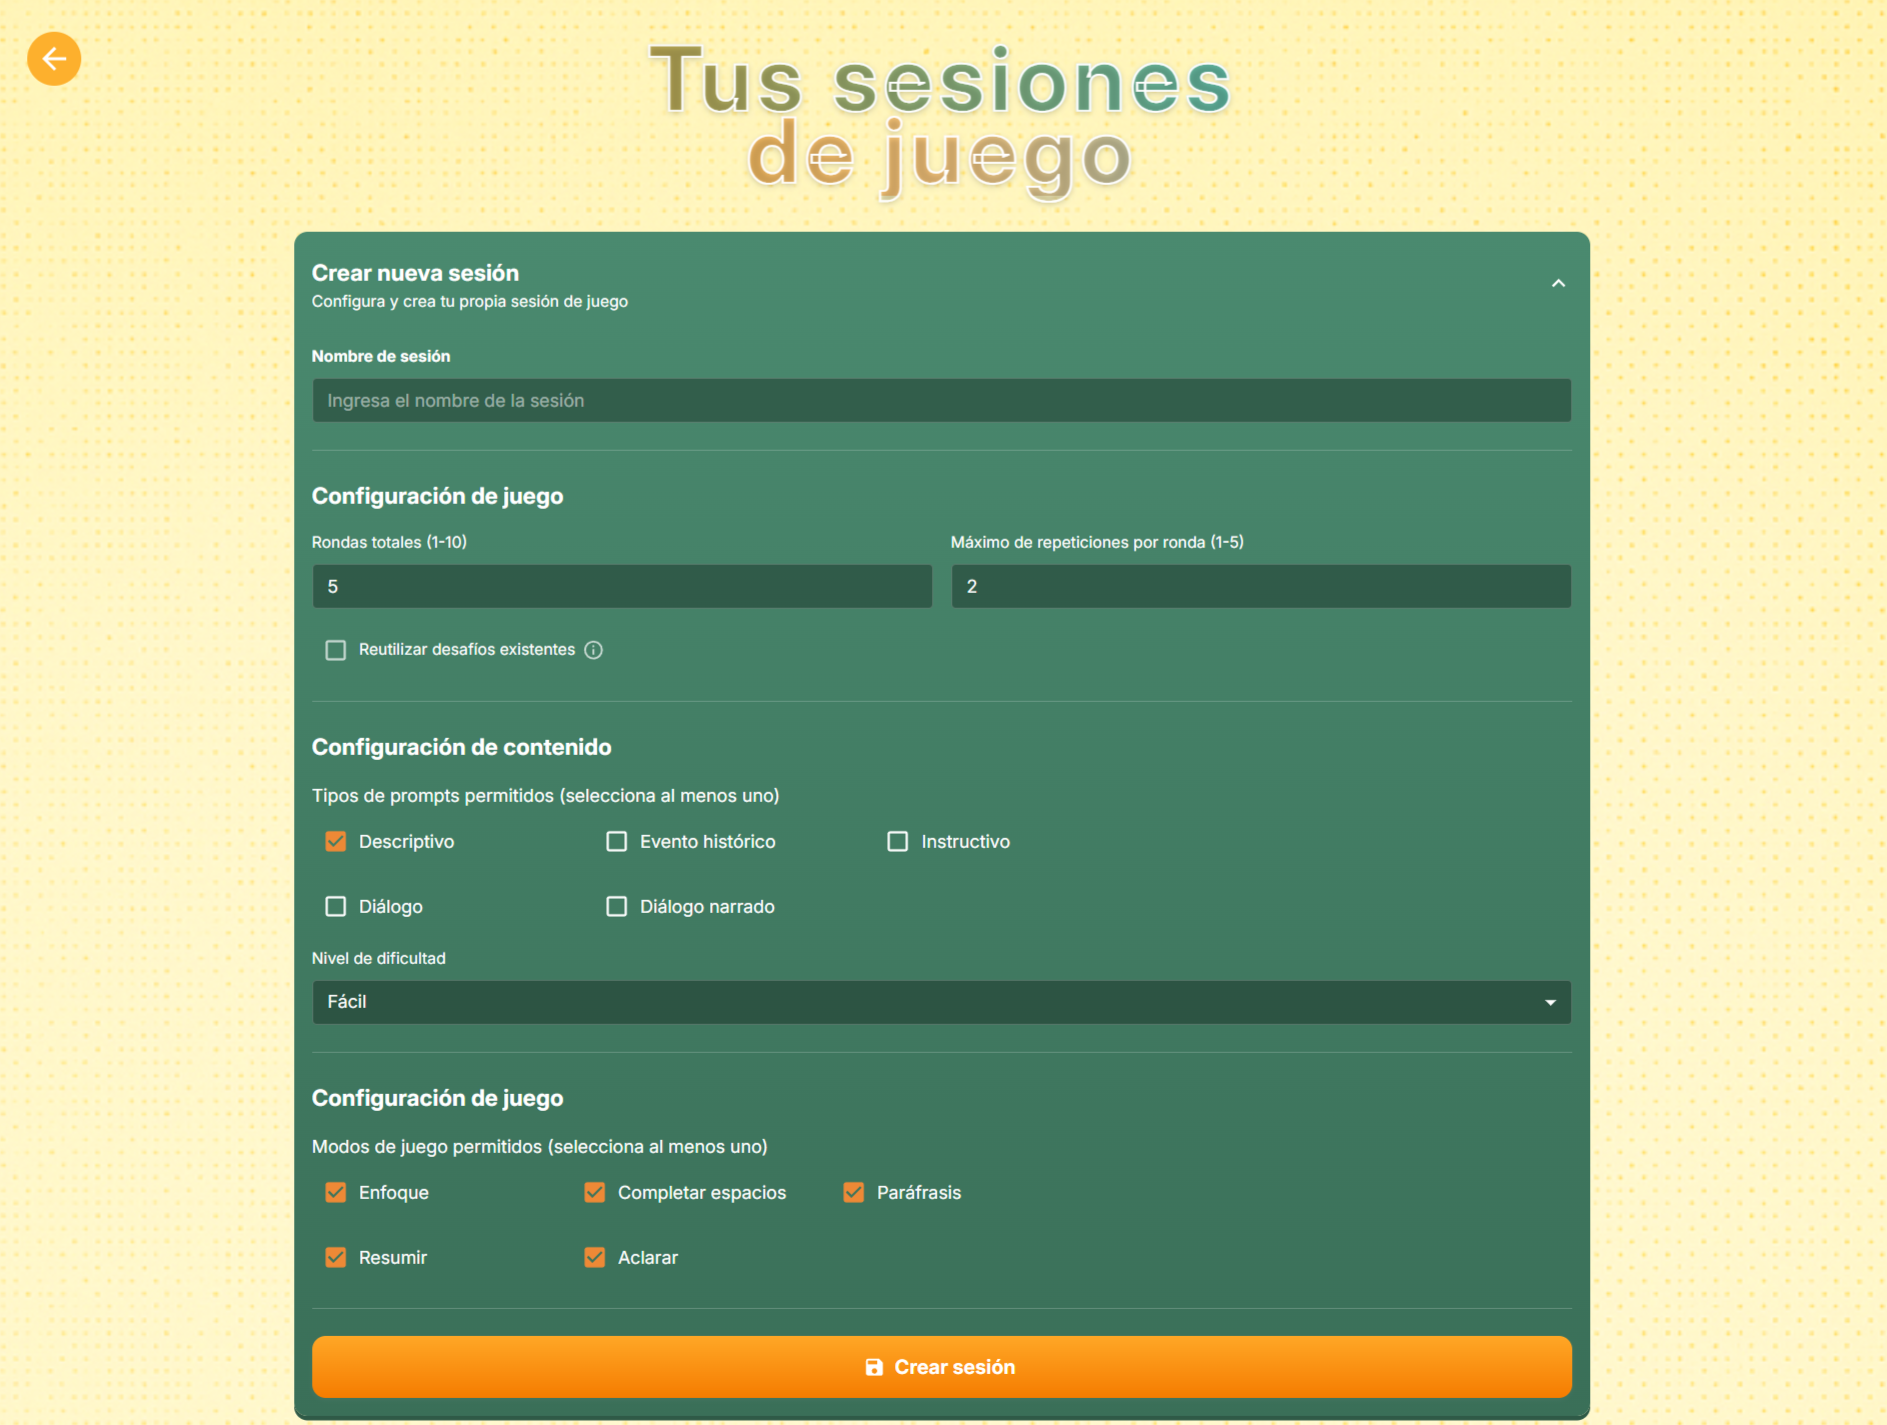
\includegraphics[width=0.95\textwidth]{Figuras/interfaces_EA/ea_crear_sesion.png}
\caption{Interfaz para la creación y configuración de una nueva sesión de juego.}
\label{fig:ea-configuracion-sesion}
\end{figure}

\noindent\textit{Descripción.}
Antes de iniciar una sesión, el estudiante define parámetros como el número total de rondas, el máximo de repeticiones por ronda, los tipos de prompts permitidos y los modos de juego habilitados. También puede decidir si desea reutilizar desafíos previamente generados.

% -------------------------------------------------
\subsection*{Listado de sesiones de juego}
% -------------------------------------------------

\begin{figure}[H]
\centering
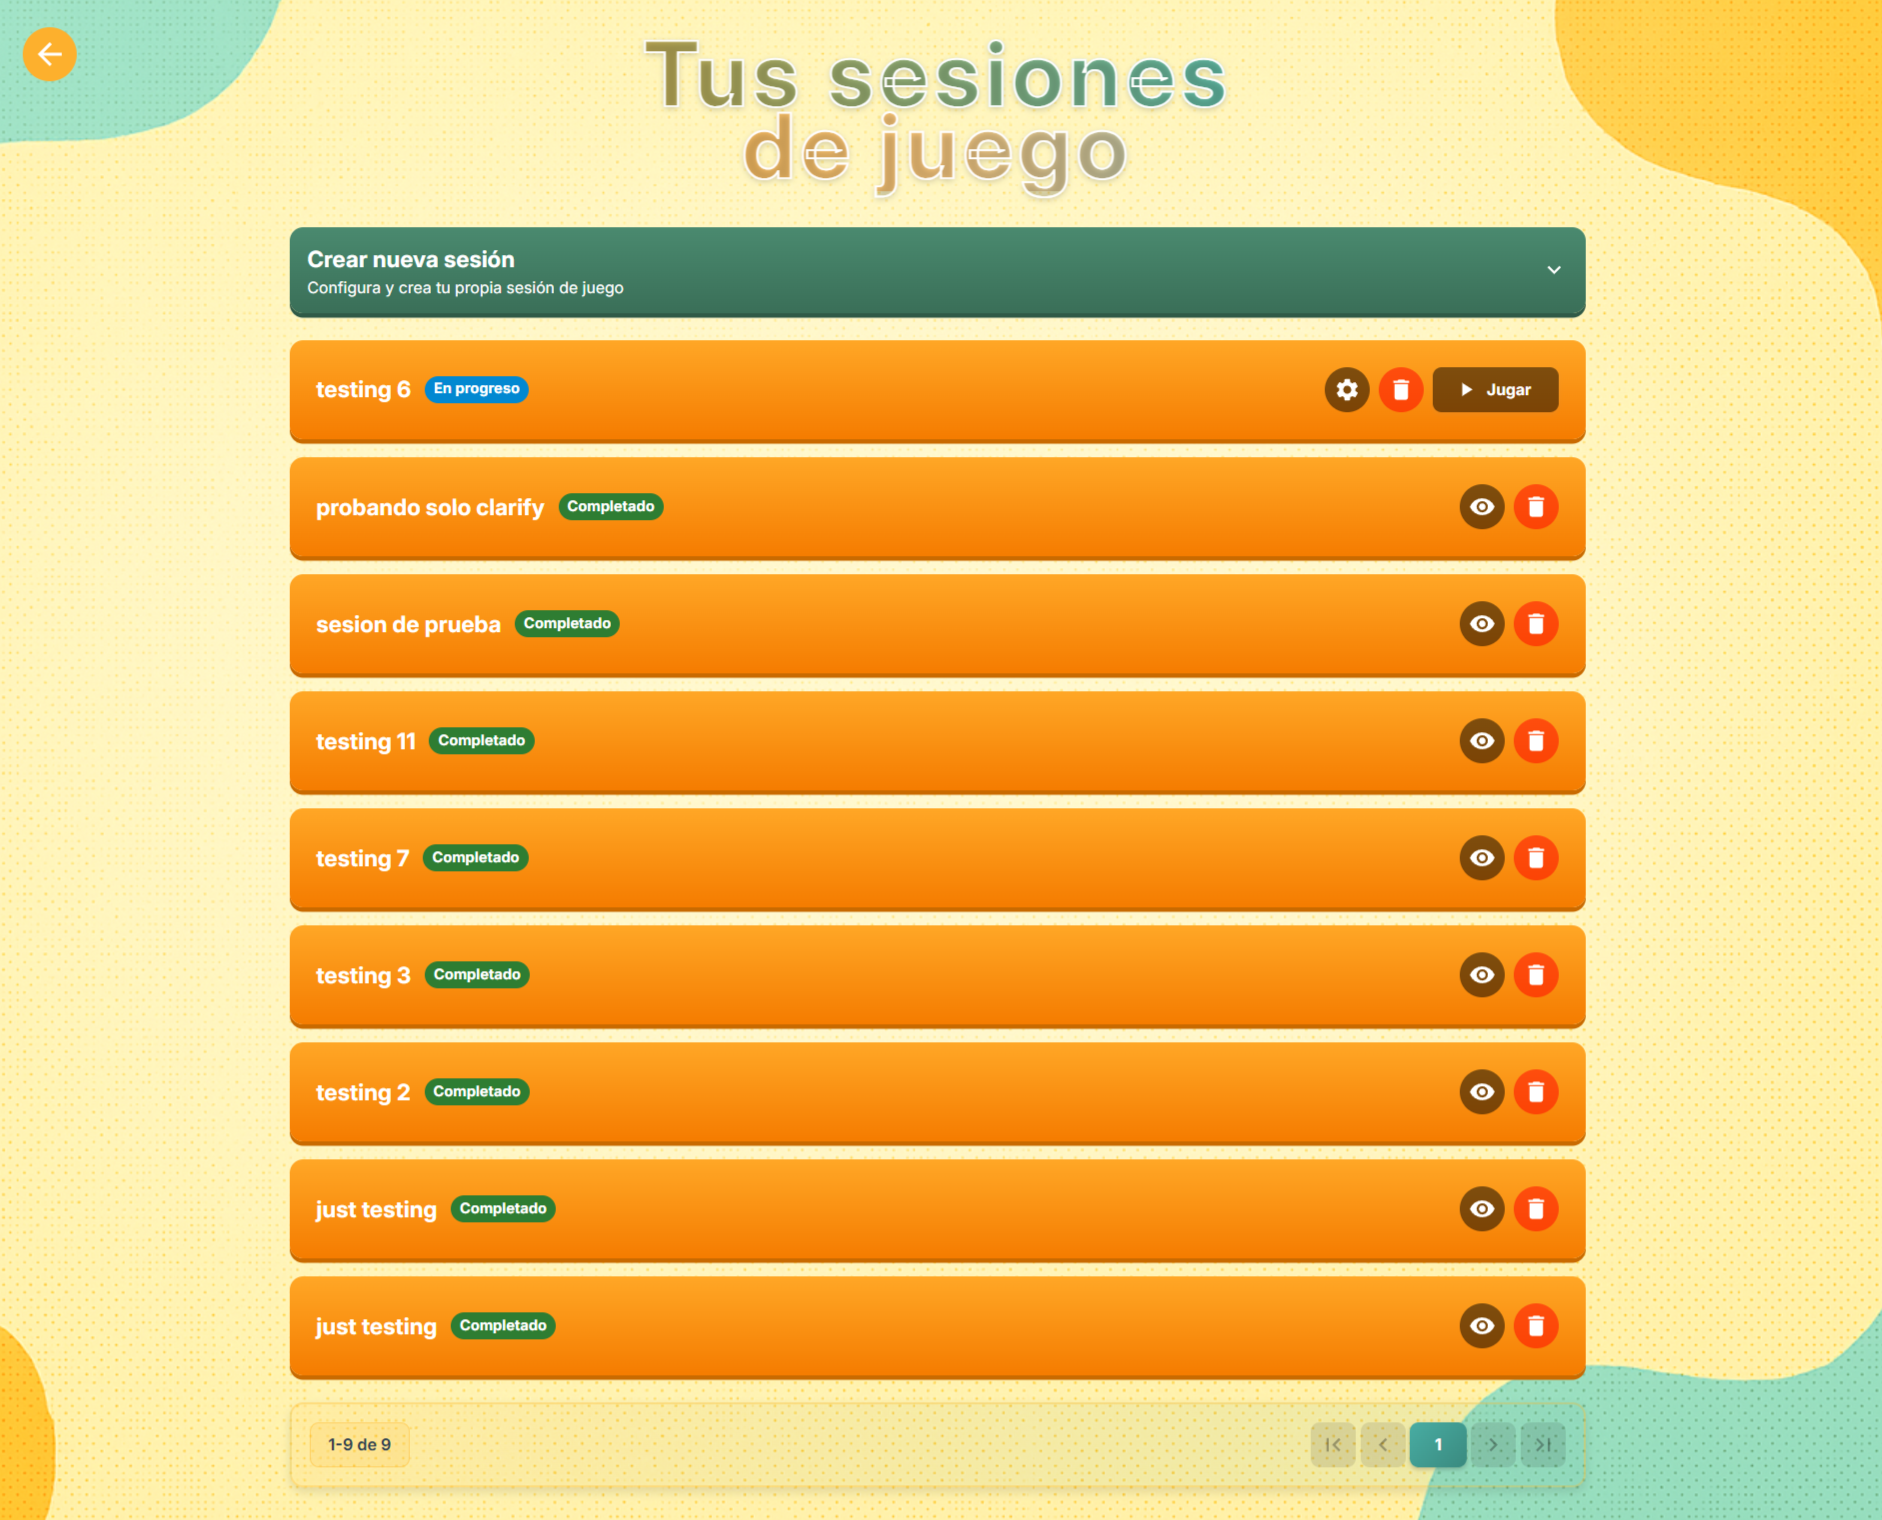
\includegraphics[width=0.95\textwidth]{Figuras/interfaces_EA/ea_listado_sesiones.png}
\caption{Listado de sesiones creadas por el estudiante, con opciones para gestionarlas o reanudar el juego.}
\label{fig:ea-listado-sesiones}
\end{figure}

\noindent\textit{Descripción.}
La vista principal muestra todas las sesiones creadas, indicando su estado (\textit{En progreso} o \textit{Completado}). Desde esta sección, el estudiante puede iniciar, continuar, revisar o eliminar sesiones existentes.

% -------------------------------------------------
\subsection*{Interacción dentro de una ronda de juego}
% -------------------------------------------------

\begin{figure}[H]
\centering
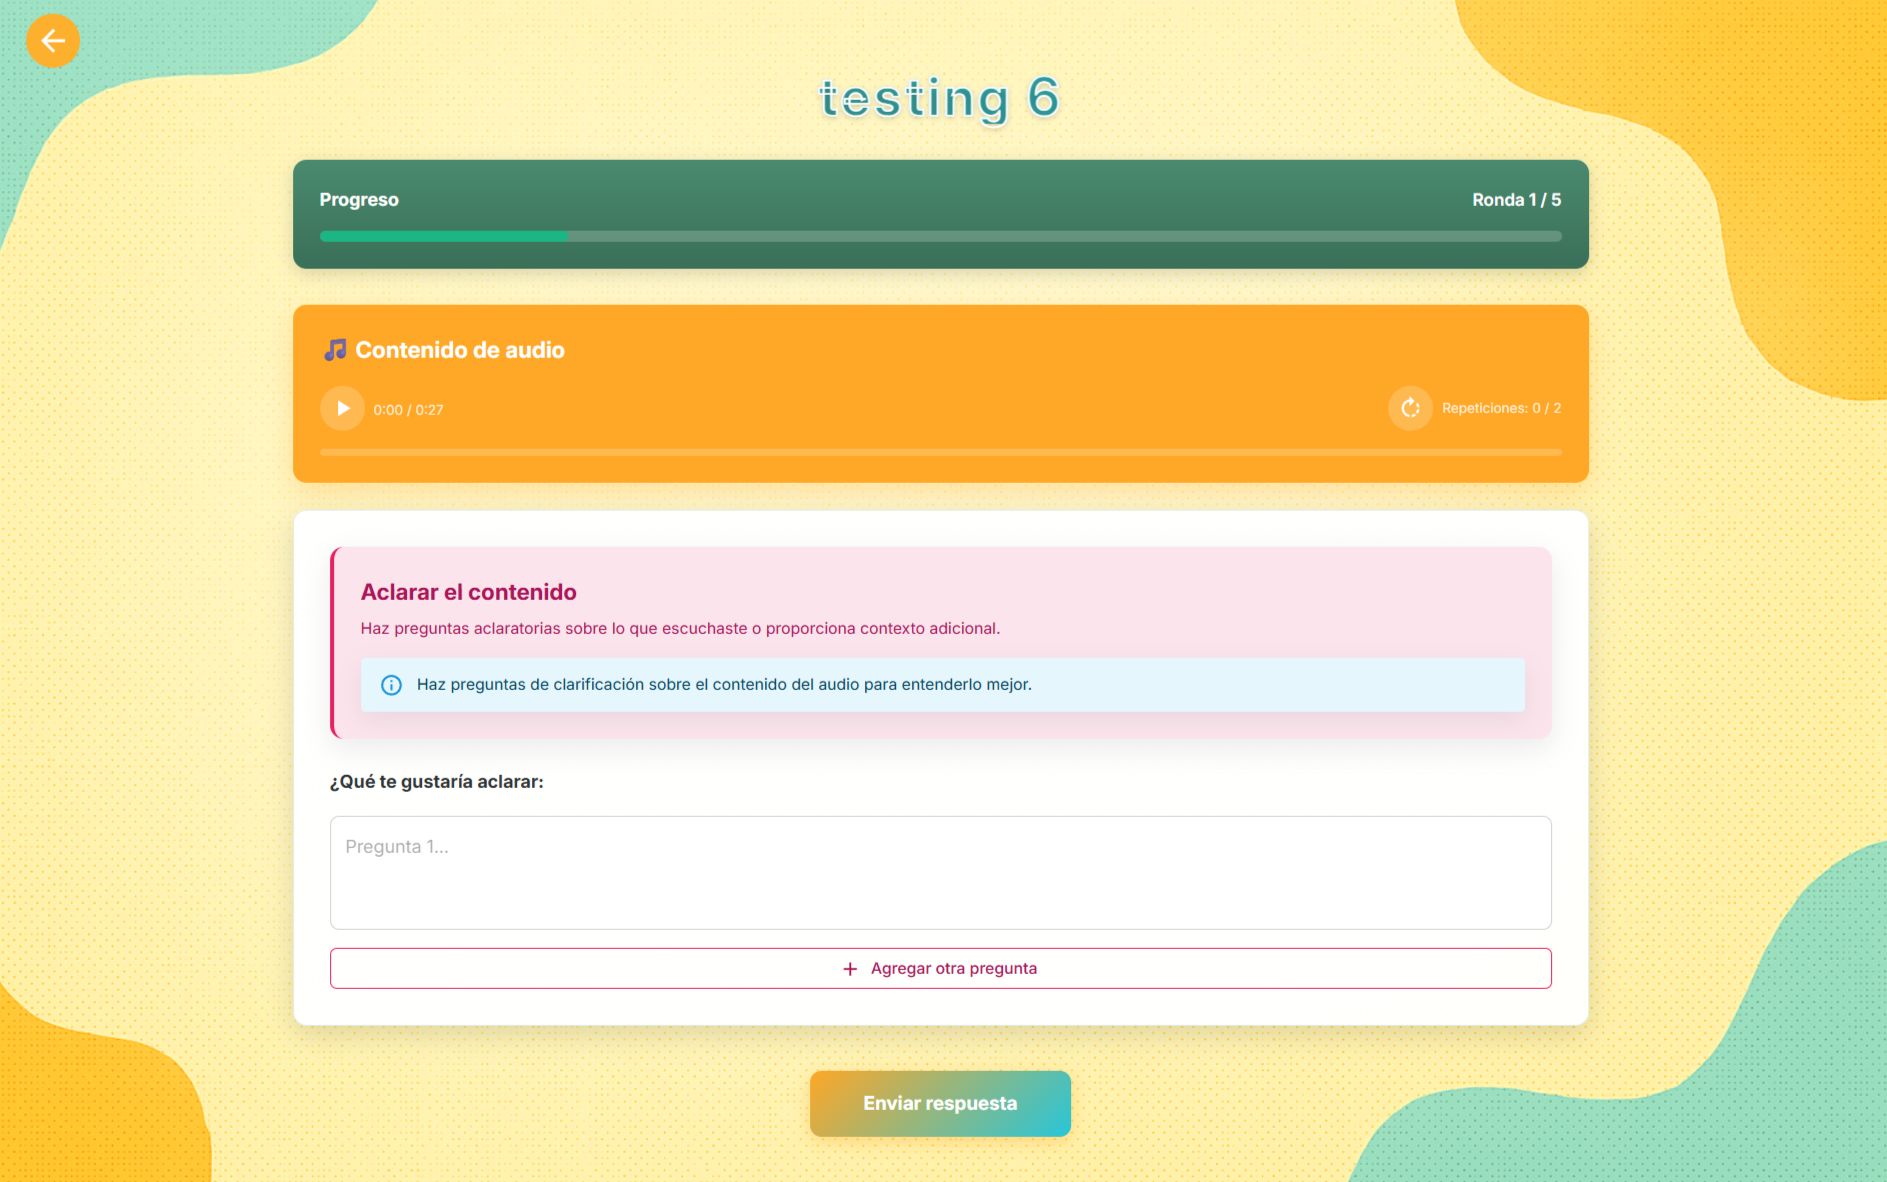
\includegraphics[width=0.95\textwidth]{Figuras/interfaces_EA/ea_ronda_juego.png}
\caption{Interfaz de una ronda activa, mostrando el audio, el conteo de repeticiones y el ejercicio asociado al modo de juego.}
\label{fig:ea-ronda}
\end{figure}

\noindent\textit{Descripción.}
Cada ronda presenta el clip de audio generado por el sistema, el número de repeticiones de reproducción utilizadas y disponibles, y el ejercicio correspondiente al modo de juego asignado (p. ej., aclarar, resumir, completar espacios). El estudiante puede volver a escuchar el audio dentro del límite permitido antes de responder, y posteriormente envía su respuesta mediante el formulario presentado.


% -------------------------------------------------
\subsection*{Evaluación y retroalimentación por ronda}
% -------------------------------------------------

\begin{figure}[H]
\centering
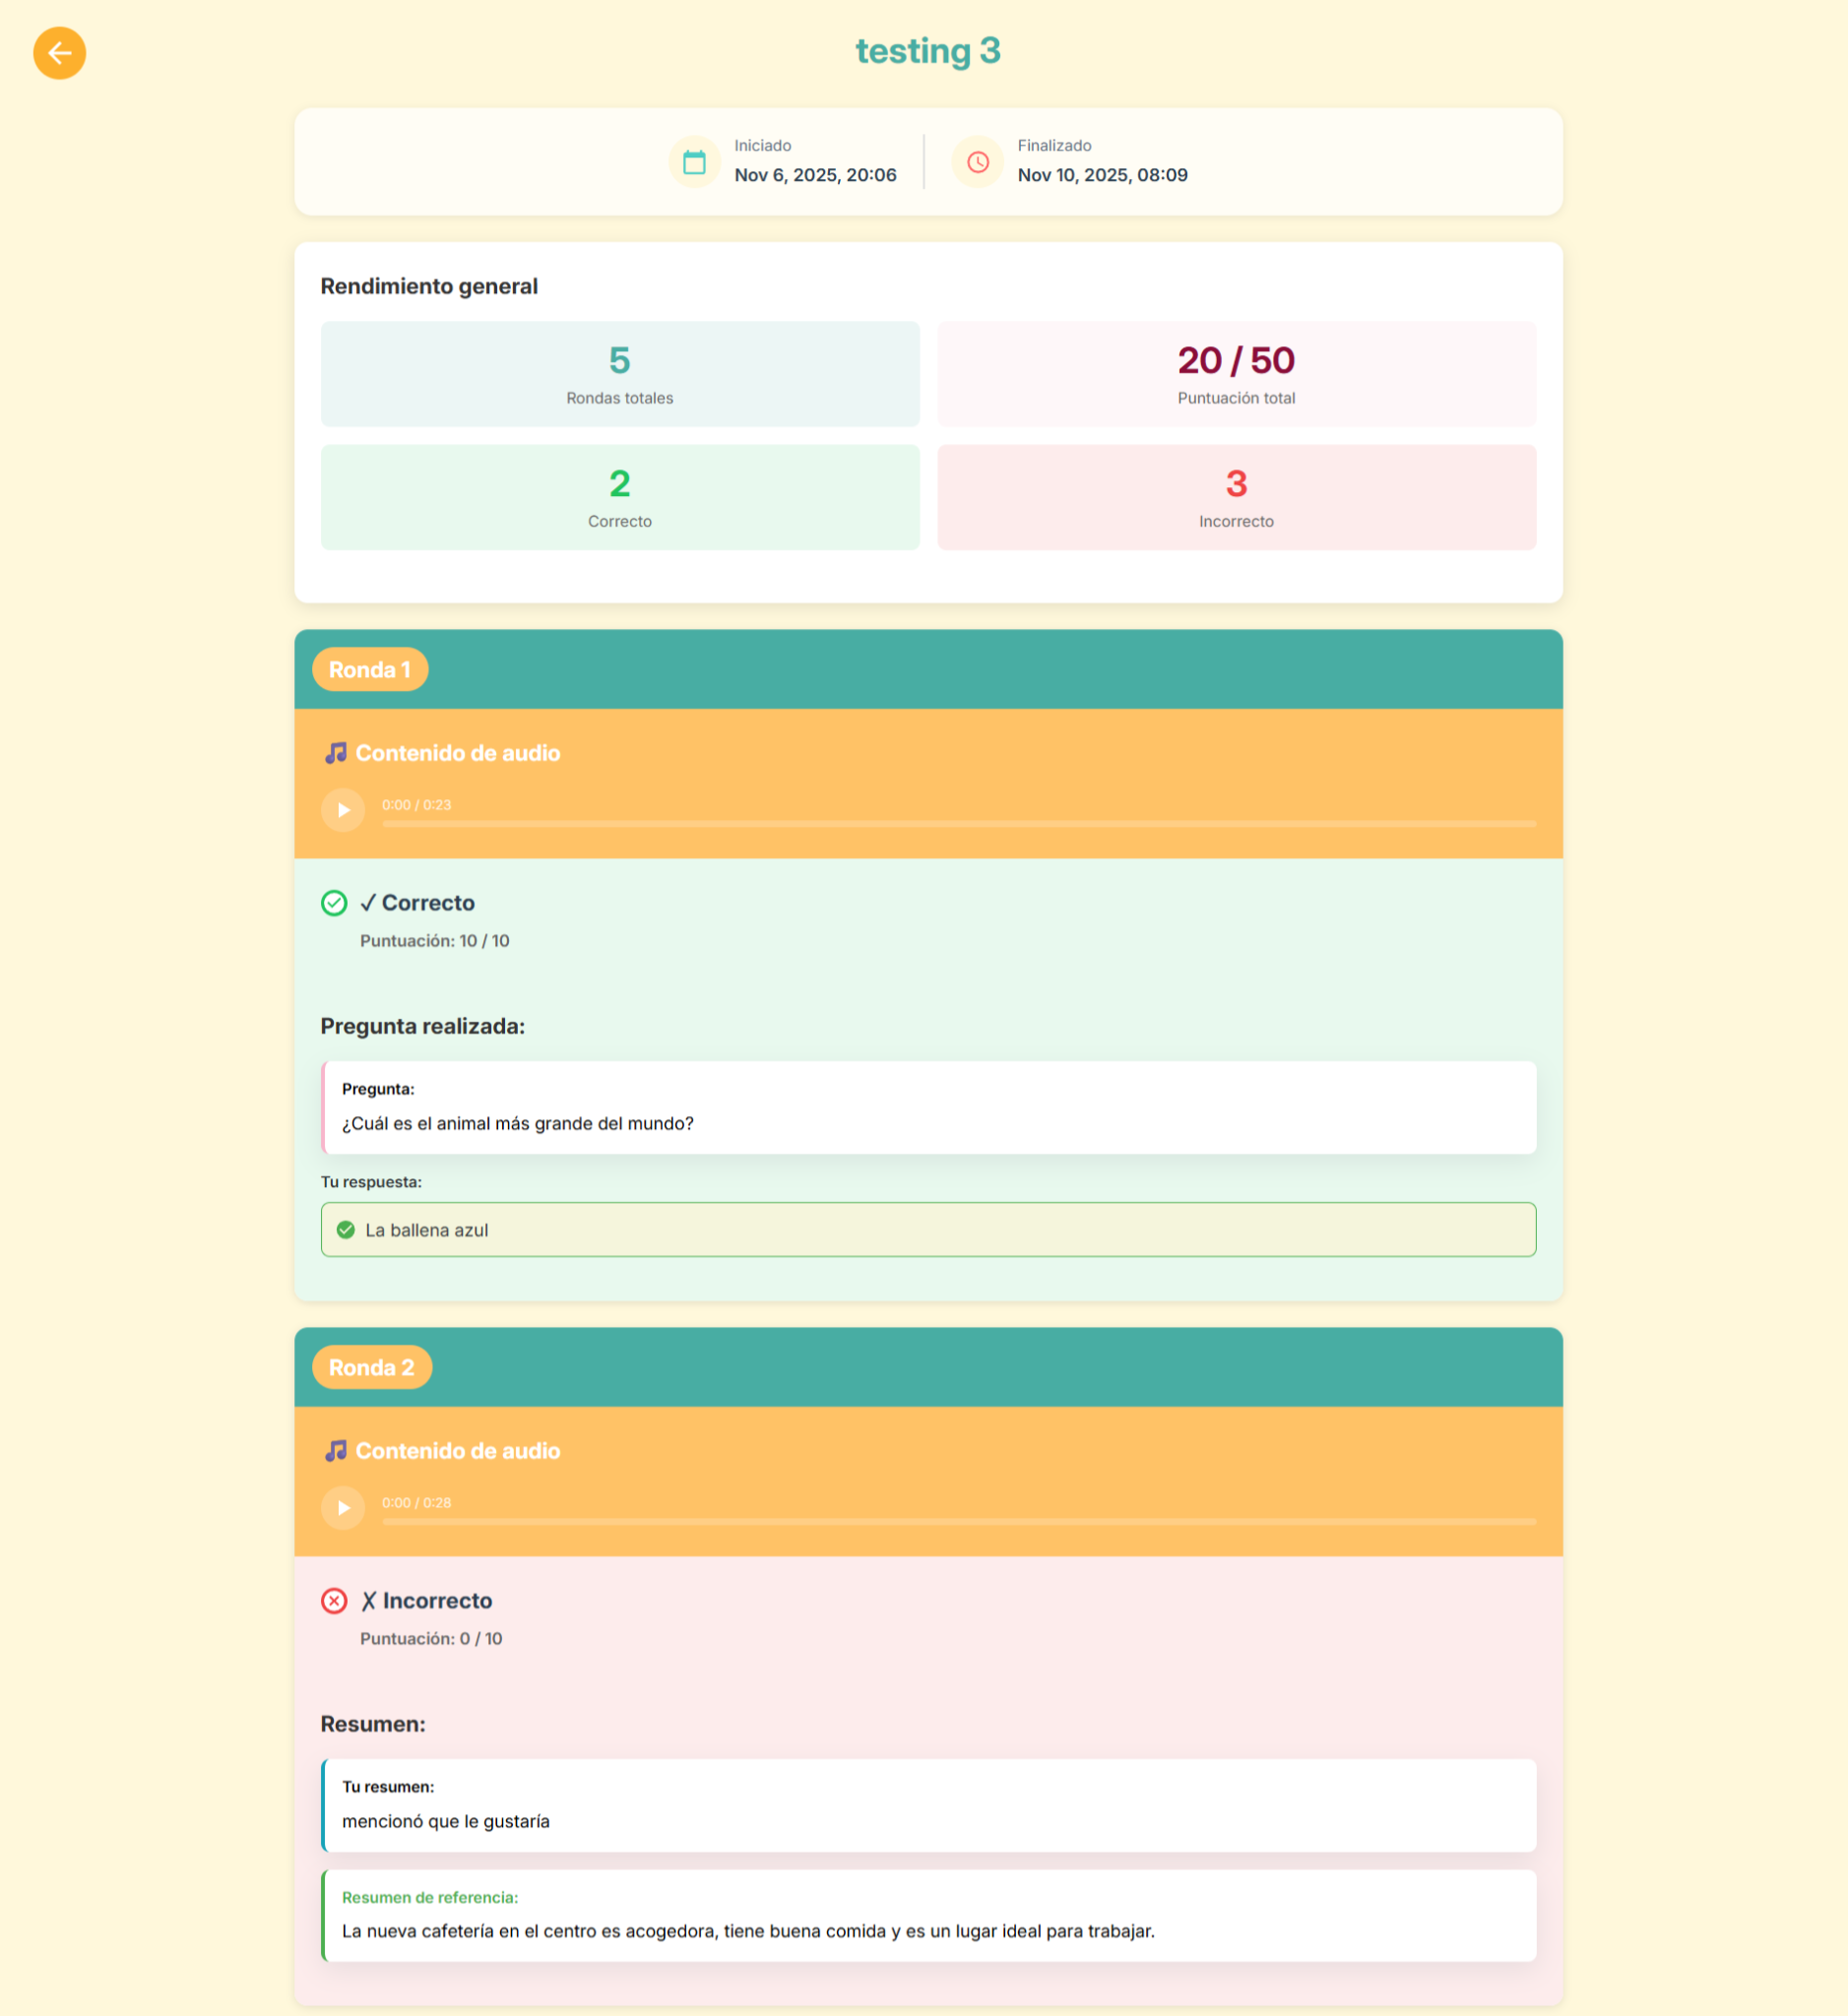
\includegraphics[width=0.95\textwidth]{Figuras/interfaces_EA/ea_reporte_sesion.png}
\caption{Reporte general de una sesión completada, con el desglose de rondas y sus resultados.}
\label{fig:ea-reporte-sesion}
\end{figure}

\noindent\textit{Descripción.}
Una vez finalizada la sesión, se presenta un informe detallado que incluye el número total de rondas, la puntuación acumulada, las respuestas correctas e incorrectas y un desglose completo de cada ronda. Cada bloque muestra el audio utilizado, la respuesta enviada, la evaluación otorgada y (cuando aplica) la comparación con la respuesta o referencia generada por el sistema.

% -------------------------------------------------
\subsection*{Detalle de ejercicios según el modo de juego}
% -------------------------------------------------

\noindent Los ejercicios correspondientes a los modos de juego \textit{Enfoque}, \textit{Completar espacios}, \textit{Paráfrasis}, \textit{Resumen} y \textit{Aclarar} se presentan directamente dentro de la interfaz de cada ronda. Dado que estas actividades se integran de manera contextualizada en la vista de ronda ya ilustrada en la Figura~\ref{fig:ea-ronda}, no se incluyen capturas adicionales. Cada ejercicio adapta dinámicamente su formato al tipo de interacción requerido por el modo de juego.


